%chapter-redistricting
\declareproblemlettering{R}
\pagestyle{fancy}

\cleartooddpage

\chapter{Redistricting}
\label{ch:district}
According to the Supreme Court, the Constitution requires that population must be equalized across districts. The idea is that if one Iowan lives in a district with 1 million other voters while another Iowan lives in a district with only 200,000 other voters, the second one's vote is more influential in choosing a member of Congress. Of course, populations shift, growing or shrinking over time.

To prevent those shifts from leaving unbalanced districts, state legislatures must redraw their electoral districts every 10 years, after the Census Bureau releases its new population data. redistricting regularly leads to heated political and legal fights as legislators scramble to gain advantage for their parties.

Once the census has been taken and all the numbers have been added up and the apportionment problem has been solved (up to the Supreme Court if necessary), it is time to divide up each state into districts (one per representative).  Some of the rules of redistricting are: \index{redistricting!rules}
\begin{itemize}
	\item Population must be equalized across districts. \vfill
	\item Each district must be (if possible) physically connected.\vfill
\end{itemize}
Additionally, each state has more rules that they have decided on.  In most states, the party in power when the census data comes out gets to draw in district lines for Federal Representatives and all state offices that need districts.  This process is done by hand often block by block.  In 2011 the new field of data science made it possible for whoever was in charge to manipulate the lines in such a way that their majority was nearly guaranteed in the near future.
 
\clearpage
\section{Gerrymandering}

\index{gerrymander}
 \begin{tabular}{m{.45\textwidth}m{.45\textwidth}}
	 The process of dividing the state into the appropriate number of districts is called redistricting, but in the popular press, it is often referred to as gerrymandering.  This is because the map-makers often decide to split things up to their benefit.  One of the earliest, most obvious examples of this was in 1812 when Massachusetts Governor Gerry and his party drew one district in such a curvy and jagged manner that the local press thought it looked like a Salamander (see Figure \ref{fig:gerrymander}) and coined the term Gerrymander. &
%\begin{wrapfigure}{r}{.5\columnwidth}
%\begin{figure}[htb]%
%\caption{The Original Gerrymander}%

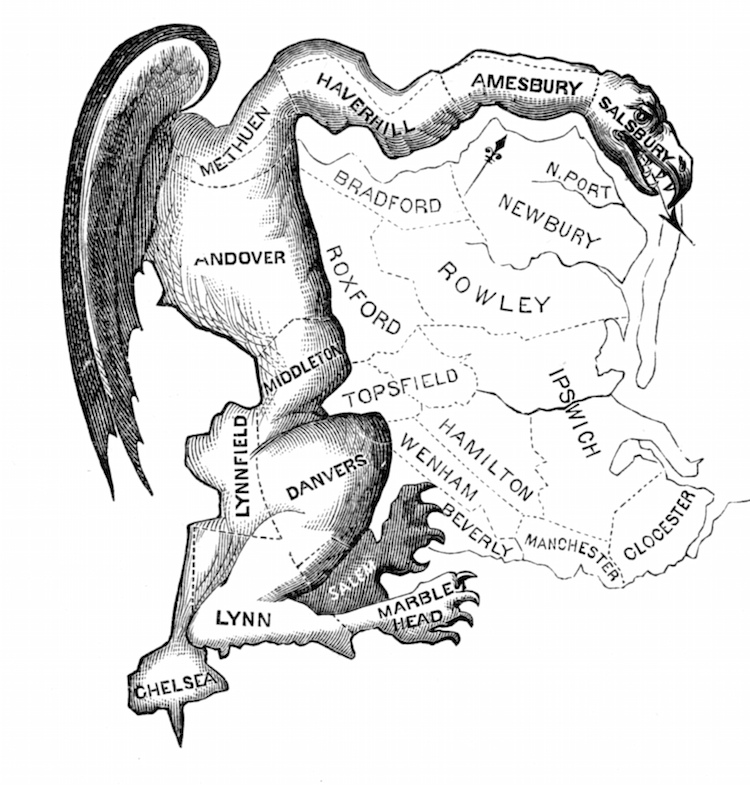
\includegraphics[width=.5\columnwidth]{gerrymander}%
\label{fig:gerrymander}%
%\end{figure}
%\end{wrapfigure}
\end{tabular}


Consider the simple state\footnote{Diagrams adapted from Stephen Nass, ``How to Steal an Election''}: 
\newcommand{\district}{
	%locations of participants
	\begin{scope}[shift = {(-.1, -.1)}]
			\draw[very thick] (0,0) -- (10,0) -- (10,5) -- (0,5) -- cycle;
	\end{scope}
	 \foreach \y in {0,1}
	 \foreach \x in {0,1,2,3,4,5,6,7,8,9}
    \draw[teal, opacity = .2, fill = teal] (\x,\y) rectangle (\x+.8,\y+.8);
	 \foreach \y in {2,3,4}
	 \foreach \x in {0,1,2,3,4,5,6,7,8,9}
    \draw[orange, fill=orange] (\x,\y) rectangle (\x+.8,\y+.8);
}

%\begin{wrapfigure}{l}{.5\columnwidth}
\begin{center}
	\begin{tikzpicture}[scale=.5]
	\district
\end{tikzpicture}
\end{center}
%\end{wrapfigure}

There are 50 people in this state who belong to two different political parties.  The census says that they should have 5 seats, so we need to divide up these people into 5 groups.  
\begin{enumerate}
	 \begin{tabular}{m{.45\textwidth}m{.45\textwidth}}
	 \item Consider the following districting of this state. Who would win with a majority of votes in each district?  Who has an advantage in the legislature?  Does it seem fair? Are the people in each district connected to each other?  Are the districts generally compact? &\newcommand{\districta}{\begin{scope}[shift = {(-.1,-.1)}]
		\draw[very thick] (0,0 ) -- (10, 0 );
		\draw[very thick] (0,1 ) -- (10, 1 );
		\draw[very thick] (0,2 ) -- (10, 2 );
		\draw[very thick] (0,3 ) -- (10, 3 );
		\draw[very thick] (0,4 ) -- (10, 4 );
		\end{scope}}
	
	\begin{tikzpicture}[scale=.5]
		\district 
		\begin{scope}[shift = {(-.1,-.1)}]
			\draw[very thick] (0,0 ) -- (10, 0 );
		\draw[very thick] (0,1 ) -- (10, 1 );
		\draw[very thick] (0,2 ) -- (10, 2 );
		\draw[very thick] (0,3 ) -- (10, 3 );
		\draw[very thick] (0,4 ) -- (10, 4 );
		\end{scope}
			\end{tikzpicture} 
	 
	\end{tabular}
	
	
	\vfill
	\clearpage
	 \begin{tabular}{m{.45\textwidth}m{.45\textwidth}}
	 \item Consider the following districting of this state. Who would win with a majority of votes in each district?  Who has an advantage in the legislature?  Does it seem fair? Are the people in each district connected to each other?  Are the districts generally compact? &
	\newcommand{\districtb}{	
	\begin{scope}[shift={(-.1,-.1)}]
					\foreach \x in {0,2,4,6,8}
	\draw[very thick] (\x,0) -- (\x, 5);

	\end{scope}
	}\begin{tikzpicture}[scale=.5]
	\district
	\districtb
	\end{tikzpicture}
	\end{tabular}
	 
	\vfill
 \begin{tabular}{m{.5\textwidth}m{.5\textwidth}}
	 \item Consider the following districting of this state. Who would win with a majority of votes in each district?  Who has an advantage in the legislature?  Does it seem fair? Are the people in each district connected to each other?  Are the districts generally compact? &
		\newcommand{\districtc}{
		\begin{scope}[shift = {(-.1, -.1)}]
				\draw[very thick] (0,0) -- (0,1) -- (1,1) -- (1,4) -- (3,4) -- (3,1) -- (4,1) -- (4,0);
				\draw[very thick] (3,4) -- (4,4) -- (4,2) -- (5, 2) -- (5,5);
				\draw[very thick] (5, 2) -- (6,2) -- (6,4) -- (9,4) -- (9, 1) -- (10, 1);
				\draw[very thick] (7,4) -- (7,1) -- (6,1) -- (6,0);
		\end{scope}
}

\begin{tikzpicture}[scale=.5]
\district
	\districtc	
	\end{tikzpicture} \end{tabular}
	 
	\vfill

	

The last diagram is an example of the `packing' and `cracking' that are illustrative of modern gerrymandering.
\begin{description}
	\item[packing] Putting a very large number of voters who all vote the same way in a single district.  In this case, the election is won by these voters, but by a very large margin.\index{gerrymander!packing}
	\item[cracking] Putting a slight majority of voters for one party in a single district.  In this case, the election is won by these voters by a slim margin.  There are a lot of minority voters in the district, but not enough to ever win an election.\index{gerrymander!cracking}
\end{description}
\clearpage

\item The state below has approximately 40\% orange (\tikz{\draw[fill=orange,orange]  circle(1ex);}) people and 60\% teal (\tikz{\draw[fill=teal,teal, opacity = .2]  circle(1ex);}) people (each color was selected randomly).  Divide the state into 10 districts in such a way so that in an election 40\% of the seats will be won by the orange people and 60\% by the teal people.

\newcommand{\firstexample}{	\begin{scope}[shift = {(-.9, -.9)}]
\draw[teal, fill = teal, opacity = 0.4] (1, 1) rectangle (1.8, 1.8);	\draw[orange, fill = orange] (1, 2) rectangle (1.8, 2.8);	\draw[orange, fill = orange] (1, 3) rectangle (1.8, 3.8);	\draw[orange, fill = orange] (1, 4) rectangle (1.8, 4.8);	\draw[teal, fill = teal, opacity = 0.4] (1, 5) rectangle (1.8, 5.8);	\draw[orange, fill = orange] (1, 6) rectangle (1.8, 6.8);	\draw[orange, fill = orange] (1, 7) rectangle (1.8, 7.8);	\draw[teal, fill = teal, opacity = 0.4] (1, 8) rectangle (1.8, 8.8);	\draw[orange, fill = orange] (1, 9) rectangle (1.8, 9.8);	\draw[orange, fill = orange] (1, 10) rectangle (1.8, 10.8);
\draw[teal, fill = teal, opacity = 0.4] (2, 1) rectangle (2.8, 1.8);	\draw[teal, fill = teal, opacity = 0.4] (2, 2) rectangle (2.8, 2.8);	\draw[teal, fill = teal, opacity = 0.4] (2, 3) rectangle (2.8, 3.8);	\draw[teal, fill = teal, opacity = 0.4] (2, 4) rectangle (2.8, 4.8);	\draw[teal, fill = teal, opacity = 0.4] (2, 5) rectangle (2.8, 5.8);	\draw[orange, fill = orange] (2, 6) rectangle (2.8, 6.8);	\draw[teal, fill = teal, opacity = 0.4] (2, 7) rectangle (2.8, 7.8);	\draw[orange, fill = orange] (2, 8) rectangle (2.8, 8.8);	\draw[teal, fill = teal, opacity = 0.4] (2, 9) rectangle (2.8, 9.8);	\draw[teal, fill = teal, opacity = 0.4] (2, 10) rectangle (2.8, 10.8);
\draw[teal, fill = teal, opacity = 0.4] (3, 1) rectangle (3.8, 1.8);	\draw[teal, fill = teal, opacity = 0.4] (3, 2) rectangle (3.8, 2.8);	\draw[teal, fill = teal, opacity = 0.4] (3, 3) rectangle (3.8, 3.8);	\draw[teal, fill = teal, opacity = 0.4] (3, 4) rectangle (3.8, 4.8);	\draw[teal, fill = teal, opacity = 0.4] (3, 5) rectangle (3.8, 5.8);	\draw[orange, fill = orange] (3, 6) rectangle (3.8, 6.8);	\draw[orange, fill = orange] (3, 7) rectangle (3.8, 7.8);	\draw[teal, fill = teal, opacity = 0.4] (3, 8) rectangle (3.8, 8.8);	\draw[teal, fill = teal, opacity = 0.4] (3, 9) rectangle (3.8, 9.8);	\draw[teal, fill = teal, opacity = 0.4] (3, 10) rectangle (3.8, 10.8);
\draw[orange, fill = orange] (4, 1) rectangle (4.8, 1.8);	\draw[teal, fill = teal, opacity = 0.4] (4, 2) rectangle (4.8, 2.8);	\draw[teal, fill = teal, opacity = 0.4] (4, 3) rectangle (4.8, 3.8);	\draw[teal, fill = teal, opacity = 0.4] (4, 4) rectangle (4.8, 4.8);	\draw[orange, fill = orange] (4, 5) rectangle (4.8, 5.8);	\draw[orange, fill = orange] (4, 6) rectangle (4.8, 6.8);	\draw[orange, fill = orange] (4, 7) rectangle (4.8, 7.8);	\draw[teal, fill = teal, opacity = 0.4] (4, 8) rectangle (4.8, 8.8);	\draw[teal, fill = teal, opacity = 0.4] (4, 9) rectangle (4.8, 9.8);	\draw[teal, fill = teal, opacity = 0.4] (4, 10) rectangle (4.8, 10.8);
\draw[teal, fill = teal, opacity = 0.4] (5, 1) rectangle (5.8, 1.8);	\draw[orange, fill = orange] (5, 2) rectangle (5.8, 2.8);	\draw[teal, fill = teal, opacity = 0.4] (5, 3) rectangle (5.8, 3.8);	\draw[teal, fill = teal, opacity = 0.4] (5, 4) rectangle (5.8, 4.8);	\draw[orange, fill = orange] (5, 5) rectangle (5.8, 5.8);	\draw[teal, fill = teal, opacity = 0.4] (5, 6) rectangle (5.8, 6.8);	\draw[teal, fill = teal, opacity = 0.4] (5, 7) rectangle (5.8, 7.8);	\draw[teal, fill = teal, opacity = 0.4] (5, 8) rectangle (5.8, 8.8);	\draw[teal, fill = teal, opacity = 0.4] (5, 9) rectangle (5.8, 9.8);	\draw[teal, fill = teal, opacity = 0.4] (5, 10) rectangle (5.8, 10.8);
\draw[orange, fill = orange] (6, 1) rectangle (6.8, 1.8);	\draw[teal, fill = teal, opacity = 0.4] (6, 2) rectangle (6.8, 2.8);	\draw[orange, fill = orange] (6, 3) rectangle (6.8, 3.8);	\draw[teal, fill = teal, opacity = 0.4] (6, 4) rectangle (6.8, 4.8);	\draw[orange, fill = orange] (6, 5) rectangle (6.8, 5.8);	\draw[teal, fill = teal, opacity = 0.4] (6, 6) rectangle (6.8, 6.8);	\draw[orange, fill = orange] (6, 7) rectangle (6.8, 7.8);	\draw[orange, fill = orange] (6, 8) rectangle (6.8, 8.8);	\draw[orange, fill = orange] (6, 9) rectangle (6.8, 9.8);	\draw[orange, fill = orange] (6, 10) rectangle (6.8, 10.8);
\draw[teal, fill = teal, opacity = 0.4] (7, 1) rectangle (7.8, 1.8);	\draw[teal, fill = teal, opacity = 0.4] (7, 2) rectangle (7.8, 2.8);	\draw[teal, fill = teal, opacity = 0.4] (7, 3) rectangle (7.8, 3.8);	\draw[teal, fill = teal, opacity = 0.4] (7, 4) rectangle (7.8, 4.8);	\draw[teal, fill = teal, opacity = 0.4] (7, 5) rectangle (7.8, 5.8);	\draw[teal, fill = teal, opacity = 0.4] (7, 6) rectangle (7.8, 6.8);	\draw[teal, fill = teal, opacity = 0.4] (7, 7) rectangle (7.8, 7.8);	\draw[orange, fill = orange] (7, 8) rectangle (7.8, 8.8);	\draw[orange, fill = orange] (7, 9) rectangle (7.8, 9.8);	\draw[teal, fill = teal, opacity = 0.4] (7, 10) rectangle (7.8, 10.8);
\draw[teal, fill = teal, opacity = 0.4] (8, 1) rectangle (8.8, 1.8);	\draw[orange, fill = orange] (8, 2) rectangle (8.8, 2.8);	\draw[teal, fill = teal, opacity = 0.4] (8, 3) rectangle (8.8, 3.8);	\draw[teal, fill = teal, opacity = 0.4] (8, 4) rectangle (8.8, 4.8);	\draw[teal, fill = teal, opacity = 0.4] (8, 5) rectangle (8.8, 5.8);	\draw[orange, fill = orange] (8, 6) rectangle (8.8, 6.8);	\draw[orange, fill = orange] (8, 7) rectangle (8.8, 7.8);	\draw[orange, fill = orange] (8, 8) rectangle (8.8, 8.8);	\draw[teal, fill = teal, opacity = 0.4] (8, 9) rectangle (8.8, 9.8);	\draw[orange, fill = orange] (8, 10) rectangle (8.8, 10.8);
\draw[teal, fill = teal, opacity = 0.4] (9, 1) rectangle (9.8, 1.8);	\draw[orange, fill = orange] (9, 2) rectangle (9.8, 2.8);	\draw[orange, fill = orange] (9, 3) rectangle (9.8, 3.8);	\draw[teal, fill = teal, opacity = 0.4] (9, 4) rectangle (9.8, 4.8);	\draw[orange, fill = orange] (9, 5) rectangle (9.8, 5.8);	\draw[orange, fill = orange] (9, 6) rectangle (9.8, 6.8);	\draw[teal, fill = teal, opacity = 0.4] (9, 7) rectangle (9.8, 7.8);	\draw[orange, fill = orange] (9, 8) rectangle (9.8, 8.8);	\draw[teal, fill = teal, opacity = 0.4] (9, 9) rectangle (9.8, 9.8);	\draw[teal, fill = teal, opacity = 0.4] (9, 10) rectangle (9.8, 10.8);
\draw[orange, fill = orange] (10, 1) rectangle (10.8, 1.8);	\draw[teal, fill = teal, opacity = 0.4] (10, 2) rectangle (10.8, 2.8);	\draw[teal, fill = teal, opacity = 0.4] (10, 3) rectangle (10.8, 3.8);	\draw[orange, fill = orange] (10, 4) rectangle (10.8, 4.8);	\draw[teal, fill = teal, opacity = 0.4] (10, 5) rectangle (10.8, 5.8);	\draw[teal, fill = teal, opacity = 0.4] (10, 6) rectangle (10.8, 6.8);	\draw[orange, fill = orange] (10, 7) rectangle (10.8, 7.8);	\draw[teal, fill = teal, opacity = 0.4] (10, 8) rectangle (10.8, 8.8);	\draw[teal, fill = teal, opacity = 0.4] (10, 9) rectangle (10.8, 9.8);	\draw[orange, fill = orange] (10, 10) rectangle (10.8, 10.8);

	\end{scope}
}
\begin{tikzpicture}[scale=.75]
	\firstexample
	\begin{scope}[]
		\draw[very thick] (0,0) -- (0,10) -- (10,10) -- (10,0) -- cycle;
	\end{scope}
\end{tikzpicture}
\vfill

\item Now, divide the same state in such a way so that 60\% of the seats will be won by the orange people.\\
\begin{tikzpicture}[scale = .75]
	\firstexample
	\begin{scope}[]
		\draw[very thick] (0,0) -- (0,10) -- (10,10) -- (10,0) -- cycle;
	\end{scope}
\end{tikzpicture}
\vfill

\end{enumerate}
%<*HWHEADER>
\clearpage
%%%%%%%%%%%%%%%%%%%%%%%%%%%%%%%%%%%%%%%%%%%%%%%%%%%%%%%%%%%%%%%%%%%%%%%%%%%%%%%%%%%%%%%%%%%%%%%%%%%%%%%%
\HOMEWORK
%</HWHEADER>

%<*HOMEWORK>


\begin{Renumerate}

  \item Consider the following map.  Put 5 districts on the map so that orange receives the most seats.
	\newcommand{\homeworkone}{
		\begin{scope}[shift = {(-.9,-.9)}]
			\draw[orange, fill = orange] (1, 1) rectangle (1.8, 1.8);	
			\draw[teal, fill = teal, opacity = 0.4] (1, 2) rectangle (1.8, 2.8);	
			\draw[teal, fill = teal, opacity = 0.4] (1, 3) rectangle (1.8, 3.8);	
			\draw[teal, fill = teal, opacity = 0.4] (1, 4) rectangle (1.8, 4.8);	
			\draw[orange, fill = orange] (1, 5) rectangle (1.8, 5.8);
			\draw[orange, fill = orange] (2, 1) rectangle (2.8, 1.8);	
			\draw[teal, fill = teal, opacity = 0.4] (2, 2) rectangle (2.8, 2.8);	
			\draw[teal, fill = teal, opacity = 0.4] (2, 3) rectangle (2.8, 3.8);	
			\draw[teal, fill = teal, opacity = 0.4] (2, 4) rectangle (2.8, 4.8);	
			\draw[teal, fill = teal, opacity = 0.4] (2, 5) rectangle (2.8, 5.8);
			\draw[teal, fill = teal, opacity = 0.4] (3, 1) rectangle (3.8, 1.8);	
			\draw[orange, fill = orange] (3, 2) rectangle (3.8, 2.8);	
			\draw[teal, fill = teal, opacity = 0.4] (3, 3) rectangle (3.8, 3.8);	
			\draw[teal, fill = teal, opacity = 0.4] (3, 4) rectangle (3.8, 4.8);	
			\draw[teal, fill = teal, opacity = 0.4] (3, 5) rectangle (3.8, 5.8);
			\draw[orange, fill = orange] (4, 1) rectangle (4.8, 1.8);	
			\draw[orange, fill = orange] (4, 2) rectangle (4.8, 2.8);	
			\draw[orange, fill = orange] (4, 3) rectangle (4.8, 3.8);	
			\draw[orange, fill = orange] (4, 4) rectangle (4.8, 4.8);	
			\draw[teal, fill = teal, opacity = 0.4] (4, 5) rectangle (4.8, 5.8);
			\draw[teal, fill = teal, opacity = 0.4] (5, 1) rectangle (5.8, 1.8);	
			\draw[teal, fill = teal, opacity = 0.4] (5, 2) rectangle (5.8, 2.8);	
			\draw[orange, fill = orange] (5, 3) rectangle (5.8, 3.8);	
			\draw[teal, fill = teal, opacity = 0.4] (5, 4) rectangle (5.8, 4.8);	
			\draw[orange, fill = orange] (5, 5) rectangle (5.8, 5.8);
	\end{scope}
}
	
\begin{center}
		\begin{tikzpicture}
		\homeworkone
		\begin{scope}
			\draw[very thick] (0,0) -- (0,5) -- (5,5) -- (5,0)  --cycle;
		\end{scope}
	\end{tikzpicture}

\end{center}	
	\item Put 5 districts on the map so that teal receives the most districts.
	
\begin{center}
			\begin{tikzpicture}
		\homeworkone
		
		\begin{scope}
			\draw[very thick] (0,0) -- (0,5) -- (5,5) -- (5,0)  --cycle;
		\end{scope}
	\end{tikzpicture}

\end{center}
\end{Renumerate} 

\ENDHOMEWORK

%%%%%%%%%%%%%%%%%%%%%%%%%%%%%%%%%%%%%%%%%%%%%%%%%%%%%%%%%%%%%%%%%%%%%%%%%%%%%%%%%%%%%%%%%%%%%

\clearpage

\section{Fairness}
The big question of the day is 
\begin{quote}
Justice Kennedy suggested, as he did in another redistricting case 13 years ago, that courts perhaps could be involved in placing limits on extremely partisan electoral maps.  13 years ago he wrote "If courts refuse to entertain any claims of partisan gerrymandering, the temptation to use partisan favoritism in districting in an unconstitutional manner will grow," 
\end{quote}

\subsection{Geometric Measures} \index{redistricting:geometric measures of fairness}
Although most states have a requirement that their districts be compact, there is no good definition for how compact a set of districts would be.  We will look at two different ways of measuring compactness.  To make measurement easier, we will be using our example districts from before.

\subsubsection{Area vs. Perimeter}
One way of measuring how compact a district is comes from dividing the area of the district by its perimeter squared and then multiplying by 16\footnote{You multiply by 16 because the Isoperimetric measure for a square is $\frac{1}{16}$ and we would like our ratio to be about 1.}.  In general, this type of calculation is known as an Isoperimetric measure. \index{redistricting!isoperimetric measure}
\begin{enumerate}
	\item Example:
\begin{center}
		\begin{tikzpicture}[scale=.5]
		begin{scope}
		 \draw[orange, fill=orange] (0,0) rectangle (.8,.8);
		\draw[orange, fill=orange] (0,1) rectangle (.8,1+.8);
		\draw[orange, fill=orange] (0,2) rectangle (.8,2+.8);
		\draw[teal, opacity = .2, fill=teal] (1,0) rectangle (1+.8, .8);
		\draw[teal, opacity = .2, fill=teal] (1,1) rectangle (1+.8, 1+.8);
			\begin{scope}[shift = {(-.1, -.1)}]
			\draw[very thick] (0,0) -- (2,0) -- (2,2) -- (1,2) -- (1, 3) -- (0,3) -- cycle;
			
			\node at (6,2) {Area = 5};
			\node at (6,1) {Perimeter = 10 };
			\node at (14,2) {Ratio $= \frac{16\cdot5}{10^2} = 0.8$};
			\end{scope}
	\end{tikzpicture}
\end{center}
 \textbf{Notes.}         \fillwithlines{\stretch{1}}

\clearpage
\begin{tikzpicture}[scale=.5]
	\begin{scope}
			\district 
			\begin{scope}[shift = {(-.1,-.1)}]
		\draw[very thick] (0,0 ) -- (10, 0 );
		\draw[very thick] (0,1 ) -- (10, 1 );
		\draw[very thick] (0,2 ) -- (10, 2 );
		\draw[very thick] (0,3 ) -- (10, 3 );
		\draw[very thick] (0,4 ) -- (10, 4 );
		\end{scope}
		\begin{scope}[shift = {(.4,.4)}]
			\node at (0,0) {\textbf{E}};
			\node at (0,1) {\textbf{D}};
			\node at (0,2) {\textbf{C}};
			\node at (0,3) {\textbf{B}};
			\node at (0,4) {\textbf{A}};
		\end{scope}
			
			\node at (5,-2) {\textbf{Redistricting Plan 1}};
	\end{scope}
	
	\begin{scope}[shift = {(4.5in,0)}]
		\district 
		\begin{scope}[shift={(-.1,-.1)}]
					\foreach \x in {0,2,4,6,8}
	\draw[very thick] (\x,0) -- (\x, 5);

	\end{scope}
	
		\begin{scope}[shift={(.4,.4)}]
			\node at (0,0) {\textbf{A}};
			\node at (2,0) {\textbf{B}};
			\node at (4,0) {\textbf{C}};
			\node at (6,0) {\textbf{D}};
			\node at (8,0) {\textbf{E}};
		\end{scope}
			
			\node at (5,-2) {\textbf{Redistricting Plan 2}};
	\end{scope}
	
	\begin{scope}[shift = {(9in,0)}]
	\district 
		\begin{scope}[shift = {(-.1, -.1)}]
				\draw[very thick] (0,0) -- (0,1) -- (1,1) -- (1,4) -- (3,4) -- (3,1) -- (4,1) -- (4,0);
				\draw[very thick] (3,4) -- (4,4) -- (4,2) -- (5, 2) -- (5,5);
				\draw[very thick] (5, 2) -- (6,2) -- (6,4) -- (9,4) -- (9, 1) -- (10, 1);
				\draw[very thick] (7,4) -- (7,1) -- (6,1) -- (6,0);
		\end{scope}
			\begin{scope}[shift = {(.4,.4)}]
				\node at (0,1) {\textbf{A}};
			\node at (0,0) {\textbf{B}};
			\node at (4,0) {\textbf{C}};
			\node at (5,2) {\textbf{D}};
			\node at (6,0) {\textbf{E}};
			\end{scope}
			
			\node at (5,-2) {\textbf{Redistricting Plan 3}};
	\end{scope}
\end{tikzpicture}

\item Calculate the area and perimeter of each district for each plan.  Fill in the table below.
\begin{center} \renewcommand{\arraystretch}{1.5}
	\begin{tabular}{|cc||cc||cc|} \hline
	Plan 1 & $16\frac{\text{Area}}{\text{Perimeter}^2}$ & Plan 2 & $16\frac{\text{Area}}{\text{Perimeter}^2}$ & Plan 3 & $16\frac{\text{Area}}{\text{Perimeter}^2}$\\\hline
	District A & & District A & &District A & \\\hline
	District B & & District B & &District B & \\\hline
	District C & & District C & &District C & \\\hline
	District D & & District D & &District D & \\\hline
	District E & & District E & &District E & \\\hline
	Average && Average && Average &\\\hline
	\end{tabular}
\end{center}

\item Does the calculation differentiate between the plans?  Does it show one plan as being ``better'' than the others?   
 \fillwithlines{\stretch{1}}

\subsubsection{Enclosing Square}
Another way of measuring how compact a district is comes from thinking of placing the district into the smallest square that contains the district.  Then you calculate the area of the district and its' enclosing square and divide the first by the second.  Generally, this type of calculation is known as a Reock measure. \index{redistricting!Reock measure}  For example:
\begin{center}
	\begin{tikzpicture}[scale=.5]
		\begin{scope}
		\draw[orange, fill=orange] (0,0) rectangle (.8,.8);
		\draw[orange, fill=orange] (0,1) rectangle (.8,1.8);
		\draw[orange, fill=orange] (0,2) rectangle (.8,2.8);
		\draw[teal, opacity = .2, fill=teal] (1,0) rectangle (1.8,.8);
		\draw[teal, opacity = .2, fill=teal] (1,1) rectangle (1.8,1.8);
			\begin{scope}[shift = {(-.1, -.1)}]
			\draw[very thick] (0,0) -- (2,0) -- (2,2) -- (1,2) -- (1, 3) -- (0,3) -- cycle;
			
			\node at (6,2) {Area = 5};
			\end{scope}
		\end{scope}
		%\node at (4in,3) {vs.};
		\node at (4in,0) {Ratio = $\frac{5}{9}=0.56$};
		\begin{scope}[shift = {(6in,0)}]
		\draw[orange, fill=orange] (0,0) rectangle (.8,.8);
		\draw[orange, fill=orange] (0,1) rectangle (.8,1.8);
		\draw[orange, fill=orange] (0,2) rectangle (.8,2.8);
		\draw[teal, opacity = .2, fill=teal] (1,0) rectangle (1.8,.8);
		\draw[teal, opacity = .2, fill=teal] (1,1) rectangle (1.8,1.8);
			\begin{scope}[shift = {(-.1, -.1)}]
			\draw[very thick] (0,0) -- (3,0) -- (3,3) -- (0,3) -- cycle;
			\node at (6,2) {Area = 9};
			
			\end{scope}
		\end{scope}
	\end{tikzpicture}
\end{center}

\item 
 \textbf{Notes.}         \fillwithlines{\stretch{1}}

\clearpage
\begin{tikzpicture}[scale=.5]
	\begin{scope}
			\district 
			\begin{scope}[shift = {(-.1,-.1)}]
		\draw[very thick] (0,0 ) -- (10, 0 );
		\draw[very thick] (0,1 ) -- (10, 1 );
		\draw[very thick] (0,2 ) -- (10, 2 );
		\draw[very thick] (0,3 ) -- (10, 3 );
		\draw[very thick] (0,4 ) -- (10, 4 );
		\end{scope}
		\begin{scope}[shift = {(.4,.4)}]
			\node at (0,0) {\textbf{E}};
			\node at (0,1) {\textbf{D}};
			\node at (0,2) {\textbf{C}};
			\node at (0,3) {\textbf{B}};
			\node at (0,4) {\textbf{A}};
		\end{scope}
			
			\node at (5,-2) {\textbf{Redistricting Plan 1}};
	\end{scope}
	
	\begin{scope}[shift = {(4.5in,0)}]
		\district 
		\begin{scope}[shift={(-.1,-.1)}]
					\foreach \x in {0,2,4,6,8}
	\draw[very thick] (\x,0) -- (\x, 5);

	\end{scope}
	
		\begin{scope}[shift={(.4,.4)}]
			\node at (0,0) {\textbf{A}};
			\node at (2,0) {\textbf{B}};
			\node at (4,0) {\textbf{C}};
			\node at (6,0) {\textbf{D}};
			\node at (8,0) {\textbf{E}};
		\end{scope}
			
			\node at (5,-2) {\textbf{Redistricting Plan 2}};
	\end{scope}
	
	\begin{scope}[shift = {(9in,0)}]
	\district 
		\begin{scope}[shift = {(-.1, -.1)}]
				\draw[very thick] (0,0) -- (0,1) -- (1,1) -- (1,4) -- (3,4) -- (3,1) -- (4,1) -- (4,0);
				\draw[very thick] (3,4) -- (4,4) -- (4,2) -- (5, 2) -- (5,5);
				\draw[very thick] (5, 2) -- (6,2) -- (6,4) -- (9,4) -- (9, 1) -- (10, 1);
				\draw[very thick] (7,4) -- (7,1) -- (6,1) -- (6,0);
		\end{scope}
			\begin{scope}[shift = {(.4,.4)}]
				\node at (0,1) {\textbf{A}};
			\node at (0,0) {\textbf{B}};
			\node at (4,0) {\textbf{C}};
			\node at (5,2) {\textbf{D}};
			\node at (6,0) {\textbf{E}};
			\end{scope}
			
			\node at (5,-2) {\textbf{Redistricting Plan 3}};
	\end{scope}
\end{tikzpicture}

\item Calculate the area and perimeter of each district for each plan.  Fill in the table below.
\begin{center} \renewcommand{\arraystretch}{1.5}
	\begin{tabular}{|cc||cc||cc|} \hline
	Plan 1 & $\frac{\text{Area District}}{\text{Area square}}$ & Plan 2 & $\frac{\text{Area District}}{\text{Area square}}$ & Plan 3 & $\frac{\text{Area District}}{\text{Area square}}$\\\hline
	District A & & District A & &District A & \\\hline
	District B & & District B & &District B & \\\hline
	District C & & District C & &District C & \\\hline
	District D & & District D & &District D & \\\hline
	District E & & District E & &District E & \\\hline
	Average && Average && Average &\\\hline
	\end{tabular}
\end{center}

\item Does the calculation differentiate between the plans?  Does it show one plan as being ``better'' than the others?   
 \fillwithlines{\stretch{1}}
\item If you were asked to chose which method better differentiates your notion of compact, which would you use and why?
\fillwithlines{\stretch{1}}

%<*HWHEADER>
\clearpage
%%%%%%%%%%%%%%%%%%%%%%%%%%%%%%%%%%%%%%%%%%%%%%%%%%%%%%%%%%%%%%%%%%%%%%%%%%%%%%%%%%%%%%%%%%%%%%%%%%%%%%%%
\HOMEWORK
%</HWHEADER>

%<*HOMEWORK>


\begin{Renumerate}

  \item Go back to the 5 districts you drew on the map (or draw new ones) so that orange receives the most seats. What is your average calculation for $\frac{16\text{area}}{\text{perimeter}^2}$?  What is your average calculation for $\frac{\text{area of district}}{\text{area of enclosing square}}$?
	\newcommand{\homeworkone}{\begin{scope}[shift = {(-.9,-.9)}]
\draw[orange, fill = orange] (1, 1) rectangle (1.8, 1.8);	\draw[teal, fill = teal, opacity = 0.4] (1, 2) rectangle (1.8, 2.8);	\draw[teal, fill = teal, opacity = 0.4] (1, 3) rectangle (1.8, 3.8);	\draw[teal, fill = teal, opacity = 0.4] (1, 4) rectangle (1.8, 4.8);	\draw[orange, fill = orange] (1, 5) rectangle (1.8, 5.8);
\draw[orange, fill = orange] (2, 1) rectangle (2.8, 1.8);	\draw[teal, fill = teal, opacity = 0.4] (2, 2) rectangle (2.8, 2.8);	\draw[teal, fill = teal, opacity = 0.4] (2, 3) rectangle (2.8, 3.8);	\draw[teal, fill = teal, opacity = 0.4] (2, 4) rectangle (2.8, 4.8);	\draw[teal, fill = teal, opacity = 0.4] (2, 5) rectangle (2.8, 5.8);
\draw[teal, fill = teal, opacity = 0.4] (3, 1) rectangle (3.8, 1.8);	\draw[orange, fill = orange] (3, 2) rectangle (3.8, 2.8);	\draw[teal, fill = teal, opacity = 0.4] (3, 3) rectangle (3.8, 3.8);	\draw[teal, fill = teal, opacity = 0.4] (3, 4) rectangle (3.8, 4.8);	\draw[teal, fill = teal, opacity = 0.4] (3, 5) rectangle (3.8, 5.8);
\draw[orange, fill = orange] (4, 1) rectangle (4.8, 1.8);	\draw[orange, fill = orange] (4, 2) rectangle (4.8, 2.8);	\draw[orange, fill = orange] (4, 3) rectangle (4.8, 3.8);	\draw[orange, fill = orange] (4, 4) rectangle (4.8, 4.8);	\draw[teal, fill = teal, opacity = 0.4] (4, 5) rectangle (4.8, 5.8);
\draw[teal, fill = teal, opacity = 0.4] (5, 1) rectangle (5.8, 1.8);	\draw[teal, fill = teal, opacity = 0.4] (5, 2) rectangle (5.8, 2.8);	\draw[orange, fill = orange] (5, 3) rectangle (5.8, 3.8);	\draw[teal, fill = teal, opacity = 0.4] (5, 4) rectangle (5.8, 4.8);	\draw[orange, fill = orange] (5, 5) rectangle (5.8, 5.8);
	\end{scope}}
	
\begin{center}
		\begin{tikzpicture}
		\homeworkone
		
		\begin{scope}
			\draw[very thick] (0,0) -- (0,5) -- (5,5) -- (5,0)  --cycle;
		\end{scope}
	\end{tikzpicture}

\end{center}	
	\item Go back to the 5 districts you drew on the map (or draw new ones) so that teal receives the most seats. What is your average calculation for $\frac{16\text{area}}{\text{perimeter}^2}$?  What is your average calculation for $\frac{\text{area of district}}{\text{area of enclosing square}}$?
	
\begin{center}
			\begin{tikzpicture}
		\homeworkone
		
		\begin{scope}
			\draw[very thick] (0,0) -- (0,5) -- (5,5) -- (5,0)  --cycle;
		\end{scope}
	\end{tikzpicture}

\end{center}

\item Does the average of $\frac{16\text{area}}{\text{perimeter}^2}$ demonstrate unfairness in either of your plans? \vfill

\item Does the average of $\frac{\text{area of enclosing square}}{\text{area of district}}$ demonstrate unfairness in either of your plans? \vfill

\end{Renumerate} 

\ENDHOMEWORK

%%%%%%%%%%%%%%%%%%%%%%%%%%%%%%%%%%%%%%%%%%%%%%%%%%%%%%%%%%%%%%%%%%%%%%%%%%%%%%%%%%%%%%%%%%%%%

\clearpage
\subsection{Arithmetic Measures}\index{redistricting!arithmetic measures of fairness}
Okay, so maybe just looking geometrically at how the districts are drawn is not a good way of testing how fair a redistricting is.  Maybe there is something about the election and where the people who live in the district are placed that would help us measure the fairness of the redistricting plan.
\subsubsection{Efficiency Gap} \index{redistricting!efficiency gap} \index{gerrymander!efficiency gap}
A state has been divided into 5 districts of 100 voters each.  Each district votes to elect a representative from one of two parties, $A$ or $B$.  In any election, many voters will end up feeling that voting was a waste of their time.  A voter could feel this way for two reasons:
\begin{itemize}
	\item Her party lost, so what was the point of showing up to vote?
	\item Her party won by a landslide, so what was the point of showing up to vote?
\end{itemize}
Corresponding to this, we will count:
\begin{itemize}
	\item All of the votes for party $A$ as wasted if party $A$ looses.
	\item All of the votes above 50\% for party $A$ as wasted if party $A$ wins.
\end{itemize}
\item Complete the following table (we will use $W_A$ as a short cut for the votes wasted by party $A$.):
\begin{center}
	\begin{tabular}{|c||c|c|p{2cm}||p{1.5cm}|p{1.5cm}||p{2cm}|p{2cm}|}\hline
	District & A votes & B votes & Winner & $W_A$ & $W_B$ & $W_A+W_B$ & $W_A-W_B$\\\hline\hline\ifsolns
	1 & 95 & 5 & A & 45 & 5 & 50 & 40\\ \hline 
2 & 40 & 60 & B & 40 & 10 & 50 & 30\\ \hline 
3 & 75 & 25 & A & 25 & 25 & 50 & 0\\ \hline 
4 & 45 & 55 & B & 45 & 5 & 50 & 40\\ \hline 
5 & 45 & 55 & B & 45 & 5 & 50 & 40\\ \hline \hline 
	TOTAL & 300 & 200 & $A$: 2 $B$:3   & 200 & 50 & 250 & 150\\\hline
		\else
	1 & 95 & 5 & $A$ & 45 & 5 & 50 & 40\\\hline
	2 & 40 & 60 &  &  &  &  & \\\hline
	3 & 75 & 25 &  &  &  &  & \\\hline
	4 & 45 & 55 &  &  &  &  & \\\hline
	5 & 45 & 55 &  &  &  &  & \\\hline \hline
	TOTAL & 300 & 200 & $A$: \hspace{.75cm} $B$:\hspace{.75cm}   &  &  &  & \\\hline\fi
	\end{tabular}
\end{center}
The \textbf{Efficiency Gap} is defined to be the fraction of the difference of wasted votes divided by the total number of votes: \index{Efficiency Gap}
\[ \text{EG} = \frac{W_A-W_B}{\text{Votes}} =\]
The $V$ in the denominator normalized EG, so that its magnitude does not depend on the population of the state.  The idea is that when EG is much larger than 0, the districting plan may be unfair to party $A$, because $A$ is wasting more votes.  When EG is much smaller than 0, then $B$ is wasting more votes, so the plan may be unfair to $B$.  We do have to be careful because if a candidate is running unopposed, the efficiency gap for that election is meaningless.  We can either throw out that district in our calculations or use data from other elections to estimate what the election would look like if the seat were contested.

\item Consider the following election

\begin{center}
	\begin{tabular}{|c||c|c|p{2cm}||p{1.5cm}|p{1.5cm}||p{2cm}|p{2cm}|}\hline
	District & A votes & B votes & Winner & $W_A$ & $W_B$ & $W_A+W_B$ & $W_A-W_B$\\\hline\hline\ifsolns
		1 & 81 & 19 & A & 31 & 19 & 50 & 12\\ \hline 
		2 & 45 & 55 & B & 45 & 5 & 50 & 40\\ \hline 
		3 & 80 & 20 & A & 30 & 20 & 50 & 10\\ \hline 
		4 & 49 & 51 & B & 49 & 1 & 50 & 48\\ \hline 
		5 & 45 & 55 & B & 45 & 5 & 50 & 40\\ \hline  \hline 
	TOTAL & 300 & 200 & $A$: 2 $B$:3   & 200 & 50 & 250 & 150\\\hline
		\else
		1 & 81 & 19 &  &  &  &  & \\ \hline 
		2 & 45 & 55 &  &  &  &  & \\ \hline 
		3 & 80 & 20 &  &  &  &  & \\ \hline 
		4 & 49 & 51 &  &  &  &  & \\ \hline 
		5 & 45 & 55 &  &  &  &  &  \\ \hline \hline
	TOTAL & 300 & 200 & $A$: \hspace{.75cm} $B$:\hspace{.75cm}   &  &  &  & \\\hline\fi
	\end{tabular}
\end{center}
Fill out the table.  

\noindent Which districts show signs of \textbf{packing}, that is putting all the voters of one party together so that, although they win the district, they have a lot of wasted votes.
 \fillwithlines{\stretch{1}}
\noindent Which districts show signs of \textbf{cracking}, that is putting just enough voters of the opposing party in the district so that they are confident of winning the election and therefore the first party has a lot of wasted votes?
 \fillwithlines{\stretch{1}}

%<*HWHEADER>
\clearpage
%%%%%%%%%%%%%%%%%%%%%%%%%%%%%%%%%%%%%%%%%%%%%%%%%%%%%%%%%%%%%%%%%%%%%%%%%%%%%%%%%%%%%%%%%%%%%%%%%%%%%%%%
\HOMEWORK
%</HWHEADER>

%<*HOMEWORK>


\begin{Renumerate}

  \item Go back to the 5 districts you drew on the map (or draw new ones) so that orange receives the most seats. Assuming that each square represents 100 voters, what is the efficiency gap for your plan?
	\newcommand{\homeworkone}{\begin{scope}[shift = {(-.9,-.9)}]
\draw[orange, fill = orange] (1, 1) rectangle (1.8, 1.8);	\draw[teal, fill = teal, opacity = 0.4] (1, 2) rectangle (1.8, 2.8);	\draw[teal, fill = teal, opacity = 0.4] (1, 3) rectangle (1.8, 3.8);	\draw[teal, fill = teal, opacity = 0.4] (1, 4) rectangle (1.8, 4.8);	\draw[orange, fill = orange] (1, 5) rectangle (1.8, 5.8);
\draw[orange, fill = orange] (2, 1) rectangle (2.8, 1.8);	\draw[teal, fill = teal, opacity = 0.4] (2, 2) rectangle (2.8, 2.8);	\draw[teal, fill = teal, opacity = 0.4] (2, 3) rectangle (2.8, 3.8);	\draw[teal, fill = teal, opacity = 0.4] (2, 4) rectangle (2.8, 4.8);	\draw[teal, fill = teal, opacity = 0.4] (2, 5) rectangle (2.8, 5.8);
\draw[teal, fill = teal, opacity = 0.4] (3, 1) rectangle (3.8, 1.8);	\draw[orange, fill = orange] (3, 2) rectangle (3.8, 2.8);	\draw[teal, fill = teal, opacity = 0.4] (3, 3) rectangle (3.8, 3.8);	\draw[teal, fill = teal, opacity = 0.4] (3, 4) rectangle (3.8, 4.8);	\draw[teal, fill = teal, opacity = 0.4] (3, 5) rectangle (3.8, 5.8);
\draw[orange, fill = orange] (4, 1) rectangle (4.8, 1.8);	\draw[orange, fill = orange] (4, 2) rectangle (4.8, 2.8);	\draw[orange, fill = orange] (4, 3) rectangle (4.8, 3.8);	\draw[orange, fill = orange] (4, 4) rectangle (4.8, 4.8);	\draw[teal, fill = teal, opacity = 0.4] (4, 5) rectangle (4.8, 5.8);
\draw[teal, fill = teal, opacity = 0.4] (5, 1) rectangle (5.8, 1.8);	\draw[teal, fill = teal, opacity = 0.4] (5, 2) rectangle (5.8, 2.8);	\draw[orange, fill = orange] (5, 3) rectangle (5.8, 3.8);	\draw[teal, fill = teal, opacity = 0.4] (5, 4) rectangle (5.8, 4.8);	\draw[orange, fill = orange] (5, 5) rectangle (5.8, 5.8);
	\end{scope}}
	
\begin{center}
		\begin{tikzpicture}[scale=.5]
		\homeworkone
		
		\begin{scope}
			\draw[very thick] (0,0) -- (0,5) -- (5,5) -- (5,0)  --cycle;
		\end{scope}
	\end{tikzpicture}
	
	\begin{tabular}{|c||c|c||p{1.5cm}|p{1.5cm}||p{2cm}|}\hline
	District & O votes & T votes & $W_O$ & $W_T$ & $W_O-W_T$\\\hline\hline
	1&&&&&\\\hline
2&&&&&\\\hline
3&&&&&\\\hline
4&&&&&\\\hline
5&&&&&\\\hline
  \hline 
TOTAL &  &  &   &  & \\\hline
	\end{tabular}

\end{center}	
	\item Go back to the 5 districts you drew on the map (or draw new ones) so that teal receives the most seats. Assuming that each square represents 100 voters, what is the efficiency gap for your plan?
	
\begin{center}
			\begin{tikzpicture}[scale=.5]
		\homeworkone
		
		\begin{scope}
			\draw[very thick] (0,0) -- (0,5) -- (5,5) -- (5,0)  --cycle;
		\end{scope}
	\end{tikzpicture}
	
		\begin{tabular}{|c||c|c||p{1.5cm}|p{1.5cm}||p{2cm}|}\hline
	District & O votes & T votes & $W_O$ & $W_T$ & $W_O-W_T$\\\hline\hline
	1&&&&&\\\hline
2&&&&&\\\hline
3&&&&&\\\hline
4&&&&&\\\hline
5&&&&&\\\hline
  \hline 
TOTAL &  &  &   &  & \\\hline
	\end{tabular}


\end{center}

\item Does the efficiency gap calculation demonstrate unfairness in either of your plans? \vfill
\end{Renumerate} 

\ENDHOMEWORK

%%%%%%%%%%%%%%%%%%%%%%%%%%%%%%%%%%%%%%%%%%%%%%%%%%%%%%%%%%%%%%%%%%%%%%%%%%%%%%%%%%%%%%%%%%%%%

\clearpage



%\subsection{Votes vs Seats}
\end{enumerate}
